%Fucking left quote symbol ` and not '    

\chapter{Quantum Chromodynamics} \label{ch:qcd}
In 1968 deep inelastic scatterings performed at the Stanford Linear Accelerator Center showed that the proton had internal structure\cite{Riordan1287} called partons at the time.  Within a decade of this discovery the partons were broken into two categories: the mass carrying fermions were known as the quarks and the gauge boson force carriers were called gluons.  The interactions of these two types of particles were described by the quantum field theory known as quantum chromodynamics (QCD) and by the SU(3) symmetry group.  SU(3) guarantees that color charge is conserved and this results in quarks grouping together into `colorless' hadrons.

\section{The QCD Lagrangian}
QCD is the strongest of the known fundamental forces.  It is a gauge field theory described by the Lagrangian density

\begin{equation}
{\cal L}=-\frac{1}{4}F^{\alpha}_{\mu\nu}F^{\mu\nu}_{\alpha}
- \alpha_{s} (\bar{q}_{j}\gamma^{\mu}T_{\alpha}q_{j})G_{\alpha}^{\mu}
+ \bar{q}_{j}(i\gamma^{\mu} \partial_{\mu} - m)q_{j}
\label{eq:lagrangian}
\end{equation}

\noindent
where $q$ and $\bar{q}$ represent the color anti-color fields summed over color $j$, $\alpha_{s}$ is the strong coupling strength,$\gamma^{\mu}$ is the Dirac gamma matrix, $G_{\alpha}^{\mu}$ is the gauge field for color \textit{$\alpha$}, is similar in analogy to the \textbf{W} matrix from the electroweak theory.  $F^{\alpha}_{\mu\nu}$ is the field strength tensor and it describes the gluon interactions. The first term of the Lagrangian is the gluon contribution and carries no mass term.  The second term of the Lagrangian describes how quarks and gluons interact with each other. The final term describes quark interactions and the coupling between them and will be explored further in this thesis.

At short distances, less than 0.2 \textit{fm}, the strong coupling constant becomes exceedingly small and second term of the Lagrangian displays an important property known as asymptotic freedom\cite{Wilczek:2005az}. 

\begin{equation}
\alpha_{s} = \frac{1}{\beta_{0} \; \ln(Q^{2}/\Lambda^{2} )}
\label{eq:alpha_s}
\end{equation}

\noindent
where $\alpha_{s}$ is the strong coupling constant, $Q^{2}$ is the momentum transfer between two interacting partons, and $\Lambda^{2}$ is a cutoff below which QCD phenomena are strongly suppressed and $\beta_{0}$ is a correction factor.

\begin{figure}[h]
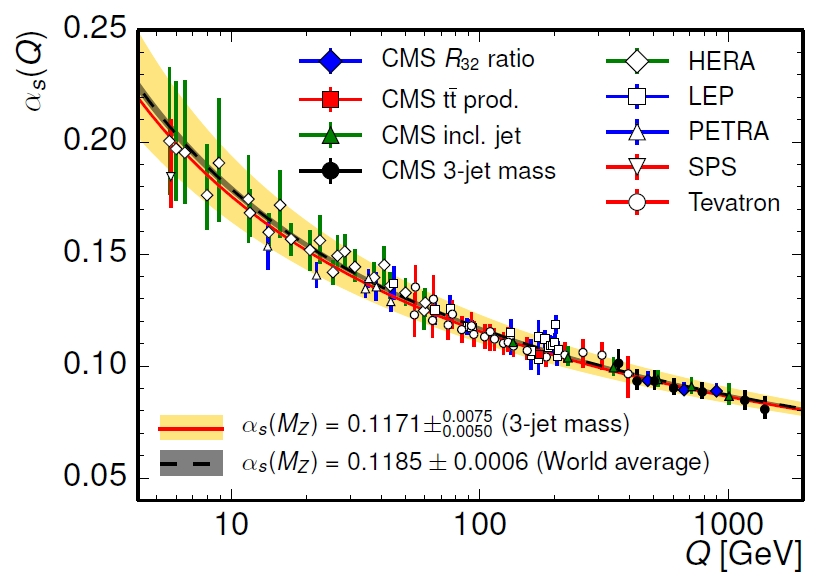
\includegraphics[width=12.0cm]{alphas_s}
\centering
\caption{Strong coupling constant ($\alpha_{s}$) as a function of the momentum transfer (Q)\cite{CMS:2014mna}.}
\label{fig:as}
\end{figure}

\section{Jets}

Hard probes (large $Q^{2}$ interactions), are produced in the earliest stages of a high energy collision when the largest momentum transfer processes occur.  As two highly energetic partons propagate away from one another, in a back-to-back fashion, they will instigate a shower of daughter partons via gluon radiation and the generation of low-mass $q \bar{q}$\, pairs.  These daughter partons will go on to form hadrons and the clustering of theses hadrons is colloquially known as a `jet'.  If the jet was created in a high energy experiment the final state hadrons will be recoreded as tracks in a tracking detector or energy deposets in a calorimeter.  This process is shown in Figure \ref{fig:MakeAJet}.



\begin{figure}[h]
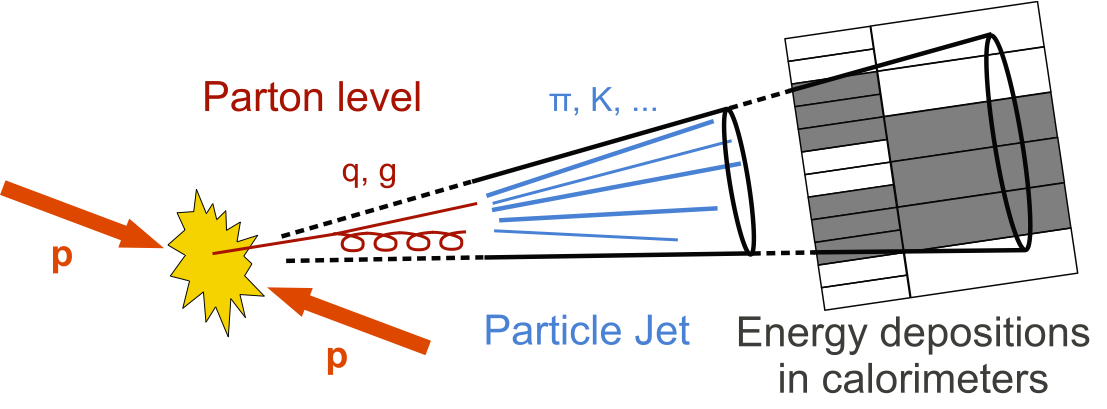
\includegraphics[width=12.0cm]{jetsatcmsand}
\centering
\caption{Diagram showing a jet created by two partons under going a hard scattering, forming into hadrons, and detected in a calorimeter\cite{JetPic}.}
\label{fig:MakeAJet}
\end{figure}

The physicist James Daniel Bjorken postulated that a correlation could be surmised by summing over the final state transverse momentum of the hadrons that form a jet to the parton that initiated the hard scattering\cite{PhysRev.179.1547}\cite{Bjorken:1973kd}.  This has lead to jets becoming the work-horse for both experimentalists and theoreticians over the past 30 years in probing QCD phenomena.  This thesis makes use of jets as an important probe of QCD and the following sections are devoted to developing a background for both the theoretical and experimental treatment of jet physics.  The following sections will be devoted to how jets are produced from a physics point-of-view and the latest results which this thesis compares to.

\subsection{Jet Production and the Factorization Theorem}

Due to confinement bare quarks are unobserved, therefore experimentalists must probe QCD interactions by detecting the color neutral final state hadrons measured in collider experiments.  Fortunately, the factorization theorem (Equation \ref{eq:xsection}) allows for the final state jet cross section to be broken into a number of steps that can either be calculated pertubativlely using pQCD or modeled phenomenologically.  Using the factorization theorem the jet cross section in a pp collision is,


\begin{equation}
d\sigma^{pp \rightarrow jet} \sim f_{a/A}(x_{1},Q^{2}) \otimes  f_{b/B}(x_{2},Q^{2}) \otimes d\sigma_{ab \rightarrow c + X} (x_{1},x_{2}) \otimes D_{c \rightarrow h/jet}(z,Q^{2})
\label{eq:xsection}
\end{equation}

\noindent
\begin{itemize}
\item  $ f_{a/A}(x_{1},Q^{2})$ and $ f_{b/B}(x_{2},Q^{2})$ are the parton distribution functions (PDF) that describe the probability of finding parton, \textit{a} or \textit{b}, within nuclei, \textit{A} and \textit{B}, with a given momentum fraction, $x = p_{parton} / p_{hadron} $ as a function of $Q^{2}$.
\item  $d\sigma_{ab \rightarrow c + X} (x_{1},x_{2})$ is the pQCD parton-parton cross section due to the hard scattering of the two partons, \textit{a} and \textit{b}, to and intermediate parton (\textit{c}).
\item   $ D_{c \rightarrow h/jet}(z,Q^{2})$ is the fragmentation function (FF) that describes the probability the an outgoing parton, \textit{c}, fragments and hardonizes into a final state hadron, \textit{h}, within a jet with momentum fraction, $z \equiv p_{hadron} / p_{parton}$.
\end{itemize}

\begin{figure}[h]
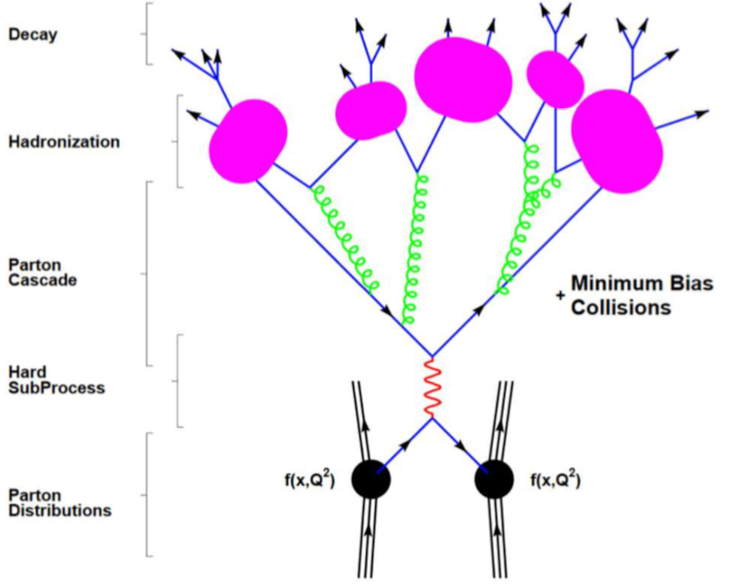
\includegraphics[width=12.0cm]{ppcollison}
\centering
\caption{Timeline of a proton-proton collision.  Starting from the bottom, two partons confined within the colliding protons have a hard interaction.  The outgoing partons will induce partonic showers by radiating quarks and gluons.  The partonic showers will eventually form into final state hadrons due to confinement which are measured in high energy experiments\cite{Dobbs:2001ck}.}
\label{fig:FactorizationCartoon}
\end{figure}

\noindent
Figure \ref{fig:FactorizationCartoon} shows a timeline of a pp collision broken into the relevant steps in accordance to the factorization theorem.  One of the best places to fundamentally test QCD phenomena using hard probes, i.e. jets, are with high energy hadron colliders such as those found at CERN\footnote{Discussed in detail in Chapter 3}, Fermilab, and BNL. The time scale that a hard probe is created in a high energy collision is on the order of $\tau \approx 1/p_{T} \approx$ \, 0.1 fm/\textit{c} which probes the initial state these interactions.  The factorization theorem allows for a high level of agreement between the QCD theory of nature and experimental observables but to ascertain this connection we should discuss each term of the factorization theorem in more depth.

\subsubsection{Parton Distribution Functions}
The PDF occurs twice in Equation \ref{eq:xsection} due to the two partons that will undergo the hard scattering being confined in two different protons.  PDFs may be thought of as conveying the structure of a nucleon in terms of the number of flavored quarks or gluons ($u(x)$, $d(x)$, $s(x)$, $\overline{u}(x)$, $\overline{d}(x)$, $\overline{s}(x)$, $g(x)$) and must obey certain constraints and summation rules.  In the case of a proton, with electric charge (\textit{e} = +1),

\begin{equation}
+1 = \frac{2}{3} \int_{0}^{1} [u(x) - \overline{u}(x)] dx - \frac{1}{3} \int^{1}_{0} [d(x) - \overline{d}(x)] dx
\label{eq:PDFcharge}
\end{equation}

\noindent
and isospin (\textit{I} = 1/2),

\begin{equation}
\frac{1}{2} = \frac{1}{2} \int_{0}^{1} [u(x) - \overline{u}(x)] dx - \frac{1}{2} \int^{1}_{0} [d(x) - \overline{d}(x)] dx
\label{eq:PDFIso}
\end{equation}

\noindent
have a solution,
\begin{equation}
 \int_{0}^{1} [u(x) - \overline{u}(x)] = 2
\label{eq:PDFSouU}
\end{equation}

\begin{equation}
\int^{1}_{0} [d(x) - \overline{d}(x)] dx = 1
\label{eq:PDFSouD}
\end{equation}

\noindent
This corresponds to the classical partonic view that protons contained two up quarks and a down quark, similarly the neutron, with charge \textit{e} = 0 and isospin I = -1/2, can be shown that it compromises two down quarks and a up quark.  Naively, we could assume that the three quarks composing a proton would each carry a momentum fraction of approximately 1/3 the total momentum of a proton.  However, high energy deep inelastic scattering experiments conducted at the Stanford Linear Collider in the 1960's\cite{Panofsky:871460} measured the momentum carried by the three quarks only accounting for about 1/2 the total proton momentum.  This lead to a more complex and dynamic model of the proton structure with the other half of the proton momentum being occupied by neutral partons which would eventually become known as gluons.

\begin{figure}[h]
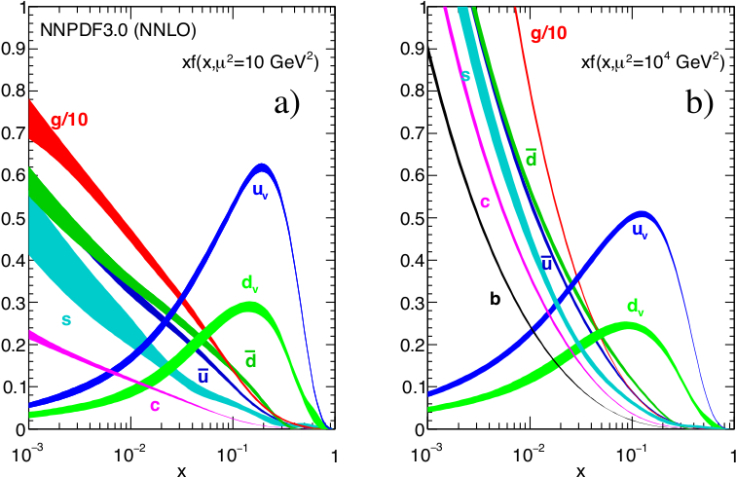
\includegraphics[width=15.0cm]{aOzz6}
\centering
\caption{Proton PDF at $Q^{2}$ = 10 GeV (left) and  $Q^{2}$ = 10 TeV (right) from the NNPDF Collaboration\cite{Feltesse:2010}.}
\label{fig:PDFNNPDF}
\end{figure}

Measuring the structure of the partons making up a nucleon is a major endeavor by both theoreticians and experimentalists.  Two of the most popular PDFs available to physicists are the CTEQ\cite{Kovarik:2013sya} (Coordinated Theoretical-Experimental Project on QCD) and the NNPDF\cite{Ball:1966481} (Neural Network Parton Distribtuion Function) sets.  Figure \ref{fig:PDFNNPDF} shows the proton PDF as a function of the momentum fraction for two energy ranges, at high values of \textit{x} the the two up quarks account for about 2/3 of the momentum fraction while down quark accounts for about 1/3 the total momentum, these quarks are collectively called the valence quarks.  At high energies, low values of \textit{x}, we see that the proton has non negligible contributions from gluons, anti-quarks, strange, and even charm quarks, these are collectively known as the sea partons.  Today, the modern picture of a protons structure is that it is mostly composed of gluons and sea quarks at low values of \textit{x} and this domination only increases as a function of $Q^{2}$\cite{Fritzsch:1992mu}.

\subsubsection{Parton-Parton Cross-Section}
The parton-parton cross section can be calculated using perturbation theory.  To the zeroth order in $\alpha_{s}$ this cross-section would be a simple quark-antiquark annihilation and would be calculable using Feynman diagrams as seen in Figure \ref{fig:qqbar}\cite{Collins:1989gx}.  Higher ordered contributions, such as the creation of virtual gluons, require the hard cross-section to be expanded as a series in terms of $\alpha_{s}$.  Calculations of the hard cross section that incorporate these higher order terms are known as \textit{next-to-leading order} (NLO) with N denoting the number of terms after the leading order that have been included in the cross-section calculation.  Various calculations of the hard cross-section of different QCD processes have been performed over the years typically using either power series or logarithmic expansions of $\alpha_{s}$\cite{Brambilla:2006wp} and corrections for LO, NLO, and even NNLO constitutes a very active field in high energy physics.

\begin{figure}[h]
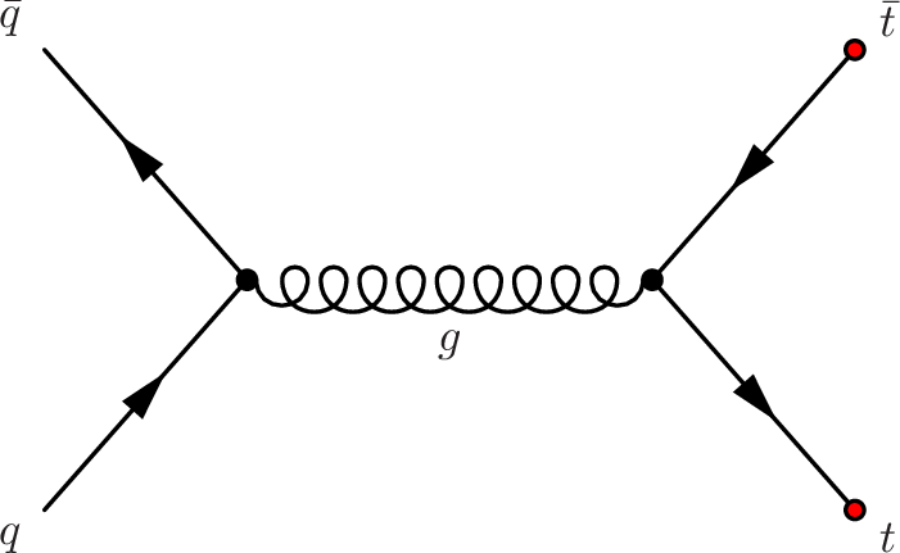
\includegraphics[width=6.0cm]{Ttbar_production_via_qqbar_annihilation}
\centering
\caption{Lowest order quark-antiquark annihilation to top-antitop pair\cite{Erdmann:2001ne}.}
\label{fig:qqbar}
\end{figure}

Perturbative techniques of the hard cross-section have been extremely successfully in describing jet features in hadronic collisions\cite{Fritzsch:1992mu}.
\subsubsection{Hadronization}

Hadronization is the process by which the colored pQCD partons of form into colorless non-pQCD hadrons and represents a significant barrier in progressing jet physics.  This is due to the fact that hadronization encompass several smaller processes which in themselves are hard to characterize. Thus, like PDFs, an accurate description of hadronization requires a phenomenological approach by which experimental results help complement theoretical calculations.  Jet production via hadronization\cite{Webber:1994zd} follows two distinct stages.  First, the partons that underwent a hard scattering start to emit radiation via gluon bremsstrahlung up until time, $t < Q^{2}$, this is known as the parton cascade.  The parton cascade is the precursor of what will become a jet as most of the radiation generated will travel in the same direction as the initial hard scattered parton.  However, this immediately poses an issue in jet physics as radiation generated at a wide angle away from the momentum axis of the inital hard scattered parton will not be associated with the jet.

\begin{figure}[h]
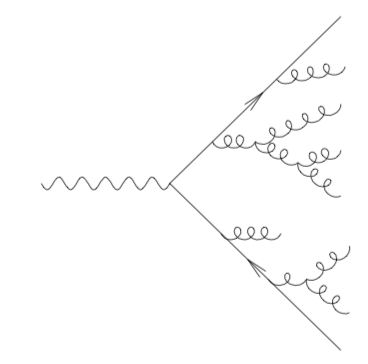
\includegraphics[width=8.0cm]{partoncascade}
\centering
\caption{Parton cascade in a hadronic collision\cite{Webber:1994zd}.}
\label{fig:pcascade}
\end{figure}

\noindent
After the cascade has ended the partons must fragment into color neutral hadrons.  Their are two main phenomenological models used to describe the hadron forming process, the Lund String Model and the Cluster Hadronization Model.  The QCD potential is,

\begin{equation}
V(r) = - \frac{\alpha_{s}}{r} + \sigma \, r
\label{eq:QCDPotential}
\end{equation}

\noindent
where the first term of Equation \ref{eq:QCDPotential} goes as the Coulomb potential with a 1/r dependence and is the dominate term at short distance and the second term has a string-like potential with $\sigma$ referring to a string-like tension.  The Lund String Model ignores gluon radiation and has fragmentation occur via breaking the string tension with the production of $q\overline{q}$ sea quarks.  The created sea quarks will carry some momentum fraction, z, of the initial parton until z falls below some cutoff.  Figure \ref{fig:qqbarstring} shows a two quarks undergoing a string breaking, each of the quarks initiating the string breaking will combine with a sea quark in an iterative manner to form hadrons.  


\begin{figure}[h]
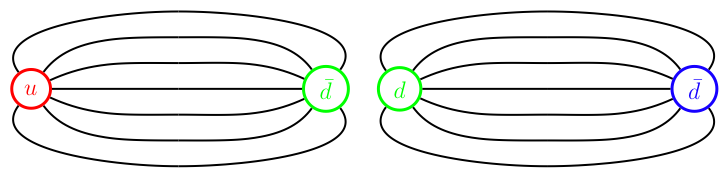
\includegraphics[width=15.0cm]{qqbarproductionvaccum}
\centering
\caption{$u \overline{d}$ generating a $d \overline{d}$ pair via string breaking which will form color neutral hadrons, black lines show the string like equipotentials.\cite{Andersson:2002ap}.}
\label{fig:qqbarstring}
\end{figure}

The Cluster Hadronization Model has gluons splitting after the parton cascade phase into $q\overline{q}$ pairs.  These pairs will form color-singlet clusters with other neighboring quarks in phase-space.  These color-singlets will typically be a few GeV/\textit{$c^{2}$} in mass and are treated as excited meson resonances.  These psuedo-resonances will decay via their normal branching ratios into the stable hadrons\cite{Webber:1983if}.


\subsubsection{Fragmentation}
Similar to how a PDF quantitatively describes the structure of a nucleon the FF quantitatively describes the hadronization process.  The FF is also similar to the PDF in that it is also a probability distribution, thus it follows the probabilistic rule that,

\begin{equation}
\sum \int z D_{c \rightarrow \, h/jet} (z,Q^{2})dz = 1
\label{eq:FFRule}
\end{equation}

\noindent
Ideally, the fractional momentum of the hadrons created from the fragmenting parton, $z \equiv p_{hadron} / p_{parton}$.  Due to the confinement of partons we must use a a suitable substitution for measuring the FF.  The Parton-Hadron Duality\cite{Jenkovszky:2012dc} states that a hadron found near the center of a jet should encompass the quantum numbers and kinematic properties associated with the hard scattered quark that initiated the jet.  Thus we can measure the fragmentation function as $z = p_{hadron} / p_{jet}$.  The formulation of the FF as a fractional energy carried by the hadrons in a jet was a breakthrough in pQCD techniques and is analogous to how an electron passing through an absorber creates photon showers with these photons generating conversion electrons until the total energy has been dissipated into the material.

\begin{figure}[h]
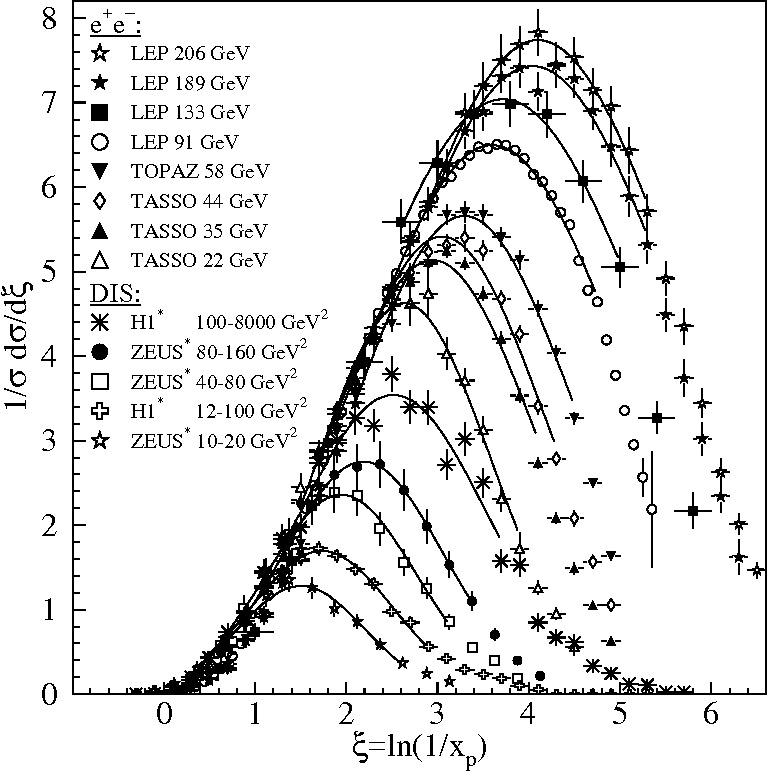
\includegraphics[width=10.0cm]{FFfunctions}
\centering
\caption{Fragmentaion Functions from $e^{+}e^{-}$and DIS experiments with fits\cite{rak_tannenbaum_2013}.}
\label{fig:FFfunc}
\end{figure}


Figure \ref{fig:FFfunc} is the FF in terms of the Gaussian equation, $z \, dN/dz = - dN /d \xi $ with $\xi = -ln  \,1/z$. The observation that the Gaussian peaks of Figure \ref{fig:FFfunc} along with the suppression of the FF at low z values due to gluon coherence were predicted by pQCD. 

\section{Jet Finding Algorithams}

A jet arises from the fragmentation of a hard parton to final state hadrons.  However, grouping the hadrons together into a jet is a non-trivial task and jet finding algorithms are deployed in order to achieve this objective.  Early on in jet physics, both theoreticians and experimentalists used a wide variety of jet finders that made comparisons between experiments or to theoretical calculations nearly impossible\cite{Atkin:2015msa}.  For example, a radiated gluon that splits into a quark anti-quark pair may become one or two jets depending on the angular separation and the algorithm used.  Early jet finders tended to be sensitive to soft particles or could give widely varying yields to the number of jets in an event.  In 1990, the Snowmass Accord\cite{Huth:217490} was held in order to standardize the definition of a jet between experimentalists and theoreticians.  The agreement maintained that any algorithm that clusters particles into a jet must be both infrared and collinear safe (IRC).  

\begin{figure}[h]
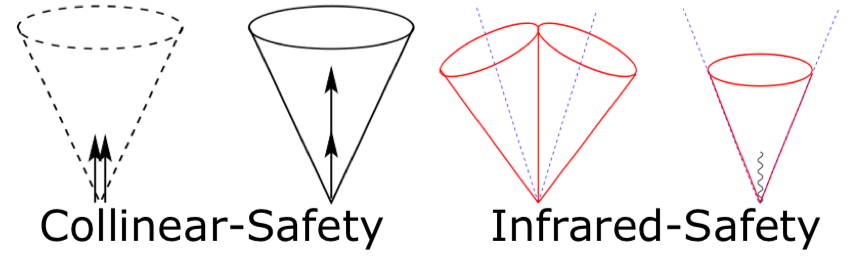
\includegraphics[width=15.0cm]{IRCsafe}
\centering
\caption{Cartoon showing Collinear and Infrared safe jet candidates\cite{Blazey:2000qt}.}
\label{fig:IRCsafe}
\end{figure}


Collinear safety ensures that a high-$p_{T}$ particle split into two or more particles should not influence the kinematics of a hard jet, this makes the jet finders insensitive to how hadrons are grouped together.  Infrared safety in turn requires that the emission of soft radiation should not affect the properties of a jet, this makes jets returned by the algorithm independent of soft physics and a true signature of a hard process.  Both of these processes are shown in Figure \ref{fig:IRCsafe}. After the adoption of these standards from the Snowmass Accord, old algorithms that violated these rules were patched and new jet finders were developed to comply with IRC safety.  The most prevalent jet finding algorithms today fall into two categories: cone algorithms and sequential recombination/clustering algorithms.

\subsection{Cone Algorithms}

Cone algorithms made up the bulk of early jet finders.  The only IRC safe cone algorithm still in use today is the seedless infra-red safe cone algorithm (SIScone).  SIScone defines a cone of radius, R, around the highest momentum particle in the coordinates of $(\eta,\phi)$\footnote{It is possible to use a Cartesian coordinate system in particle colliders, with the z-component referring to points along the beam axis while the xy-plane is perpendicular to the beam axis.  However, this system is not invariant under a Lorentz boost.  Therefore it is more useful to use the cylinrical-like coordinates of psuedorapidity ($\eta$) and the azimuth angle ($\phi$). Psuedorapidity may be thought of as the polar angle in a cylindrical coordinate system with $\eta = 0$ when the polar angle is perpendicular to the beam axis and $\eta = \inf$ along the beam axis.  $\phi$ is the azimuth angle that rotates around the beam axis.  Both, $\eta$ and $\phi$ are invariant for Lorentz boosts along the beamline and allow for easy comparisons between the center-of-mass frame and the laboratory frame of a high energy collision.}, this is the proto-jet.  SIScone then proceeds through an iterative process of finding all the particles withing the jet radius such that $R \leq \sqrt{\phi^{2} + \eta^{2}}$ and calculates a new jet center based on these particles momenta and a new weighted jet axis$(\eta,\phi)$.  If the new center matches the proto-jet center, the proto-jet is tagged as a stable jet, all the particles in that jet are removed, and SIScone moves onto the next highest $p_{T}$ particle.  Cone algorithms tend to be unpopular due to being computationally expensive, they are hard to implement theoretically, and can give results not calculable in pertubation theory.

\subsection{Sequential/Recombination Algorithms}

The other class of jet finders are the sequential/recombination algorithms, which are favored by experimentalists, theoreticians and are IRC safe.  There are three types of sequential/recombination algorithms: $k_{T}$, Anti-$k_{T}$, and the Cambridge/Aachen jet finders, with $k_{T}$ referring to the transverse momentum of particle.  All of the algorithms use a similar method, first they find the distance between every pair of particles, $d_{i,j}$,  such that



\begin{equation}
d_{i,j} = min[p^{a}_{T,i},p^{a}_{T,j}] \, \frac{\Delta^{2}_{ij}}{R^{2}}
\label{eq:JetAlgo}
\end{equation}

\noindent
where $p^{a}_{T,i}$ is the transverse momentum of particle \textit{i}, \textit{a} is free parameter that is set based on which algorithm is used, $\Delta^{2}_{ij} = (\eta_{i} - \eta_{j})^{2} + (\phi_{i} + \phi_{j})^{2}$ is the distance between the particles, and R is the radius of the jet.  A second distance is defined in the sequential/recombination algorithm scheme,

\begin{equation}
d_{i,B} = p^{a}_{T,i}
\label{eq:MinJet}
\end{equation}

\noindent
this is the distance between a given particle \textit{i} and the beam axis.  Sequential/Recombination algorithms find the set of all particles, ${d_{i,j},d_{i,B}}$, such that if $d_{i,B}$ is the minimum for particle \textit{i} it is tagged as a jet and removed from the list.  If $d_{i,j}$ are a minimum for particles \textit{i} and \textit{j} these two particles are merged together into a new particle (\textit{ij}) and a new minimum is found between (\textit{ij}) and particle \textit{k} until all the particles are either merged into jets or the minimization function is no longer satisfied.

\subsubsection{$k_{T}$ Algorithm}
The $k_{T}$ algorithm sets the value \textit{a} to 2, this results in a minimization function,

\begin{equation}
d_{i,j} = min[p^{2}_{T,i},p^{2}_{T,j}] \, \frac{\Delta^{2}_{ij}}{R^{2}}
\label{eq:kt}
\end{equation}

\noindent
which clusters low momentum particles first, making this algorithm susceptible to the underlying event (UE) or pile-up (PU).  Thus the $k_{T}$ algorithm is good at estimating any background present in a high energy collision. 

\subsubsection{Anti-$k_{T}$ Algorithm}
The Anti-$k_{T}$ algorithm sets the value \textit{a} to -2, resulting in a minimization function,

\begin{equation}
d_{i,j} = min \Bigg [\frac{1}{p^{2}_{T,i}}, \frac{1}{p^{2}_{T,j}} \Bigg ] \, \frac{\Delta^{2}_{ij}}{R^{2}}.
\label{eq:Akt}
\end{equation}

The minimization function is dominated by high-$p_{T}$ particles, thus the area and axis of a jet is only slightly perturbed by soft particles.  This makes the Anti-$k_{T}$ algorithm robust in jet finding with events having a UE and PU.  The Anti-$k_{T}$ algorithm is the default jet finding algorithm used at the Large Hadron Collider and is the one used in this thesis.

\subsubsection{Cambridge/Aachen Algorithm}

The Cambridge/Aachen algorithm sets \textit{a} to 0 and this results in a minimization function of,

\begin{equation}
d_{i,j} = \frac{\Delta^{2}_{ij}}{R^{2}}
\label{eq:CBalg}
\end{equation}

\noindent
which makes it independent of particle momentum and sensitive to PU and UE.  Due to the fact that the Cambridge/Aachen algorithm is only dependent on the particle coordinate it is most useful in studying jet structure.

\begin{figure}[h]
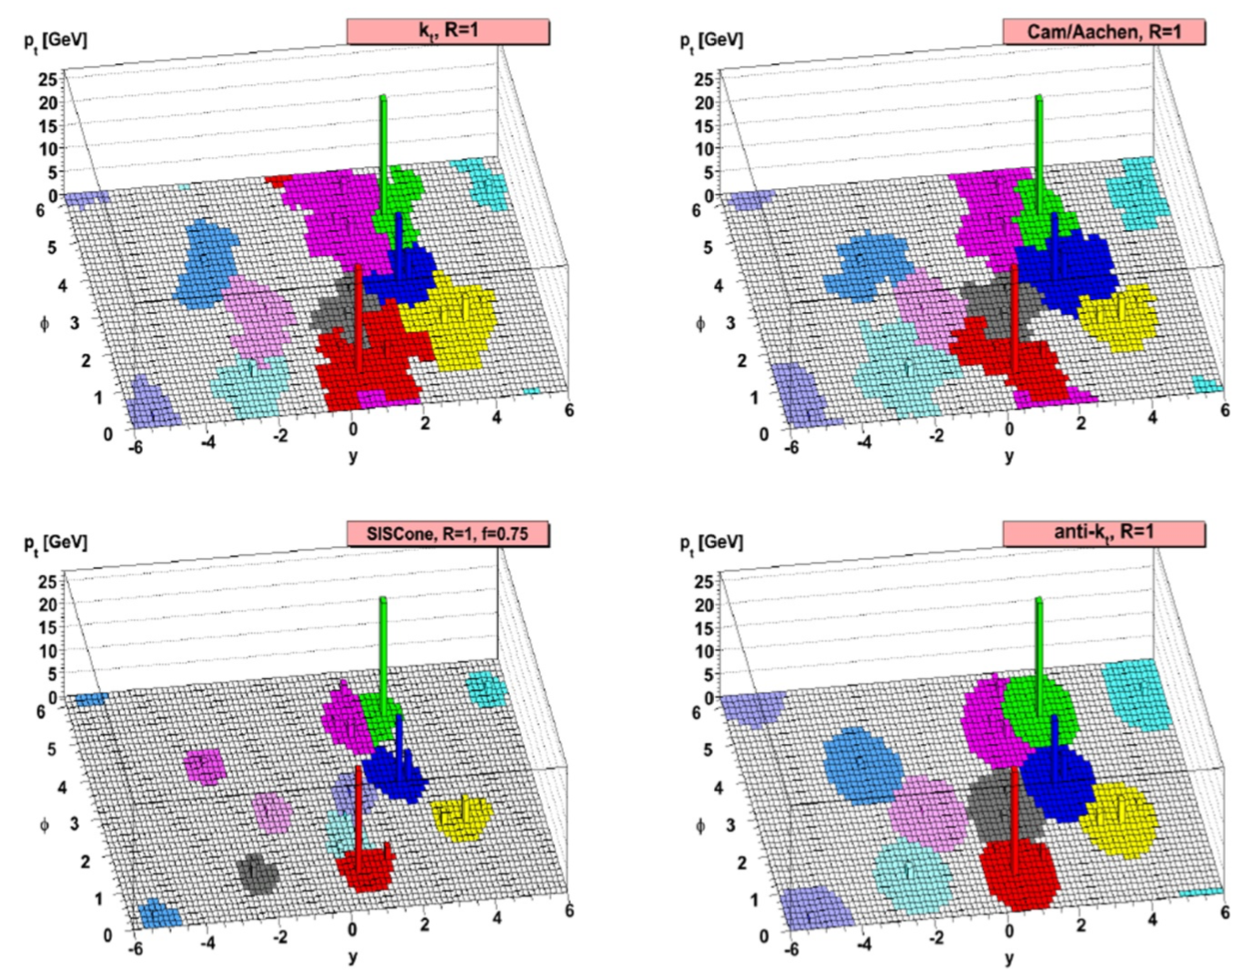
\includegraphics[width=15.0cm]{FastJet}
\centering
\caption{Lego plot of all four jet finders used on a single event with R = 1 jet radius\cite{Atkin:2015msa}.}
\label{fig:AllJetFinder}
\end{figure}

Figure \ref{fig:AllJetFinder} shows the jets found in a single event using all four jet finding algorithms.  It should be noted that the Cambridge/Aachen and $k_{T}$ algorithms have highly irregular and large shapes, making them both susceptible to the presence of a UE, while SIScone finds an additional jet due to splitting.  The Anti-$k_{T}$ algorithm finds circular jets which demonstrates its robustness to hard radiation.  

Once a stable jet is found, a recombination scheme is deployed in order to garner the jet kinematics.  By adding the 4-vector, $\boldsymbol{p}^{\mu} = (\boldsymbol{E},\boldsymbol{p}_{x},\boldsymbol{p}_{y},\boldsymbol{p}_{Z})$, for all of the associated particles composing a jet, we may obtain the jet momentum, energy, coordinates, etc\footnote{For a review of relativistic kinematic see Appendix ...}.  In a particle collider with the tracks from a tracking detector measuring particle momentum and the towers of a calorimeter measuring particle energy we obtain the following relationships



\begin{equation}
p_{T}^{jet} = \sum_{particles} p_{T} = \sum_{tracks} p_{T}
\label{eq:JePt}
\end{equation}

\begin{equation}
E^{jet} = \sum_{particles} E = \sum_{towers} E
\label{eq:JetE}
\end{equation}

\begin{equation}
\eta^{jet} = \frac{1}{2} \, \ln \Bigg (  \frac{|\boldsymbol{p}^{jet}| + p_{L}^{jet}}{|\boldsymbol{p}^{jet}| - p_{L}^{jet}}  \Bigg )
\label{eq:JetEta}
\end{equation}

\begin{equation}
\tan \phi^{jet} = \frac{p_{y}^{jet}}{p_{x}^{jet}}
\label{eq:JetPhi}
\end{equation}
\noindent 
where $p_{L}$ refers to the longitudinal momentum which is the momentum component parallel to the beam axis.  This method of adding the 4-vector of the particles composing the jet together in order to gain the jet kinematics is known as the E-scheme\cite{Cacciari:2011ma}.

\subsection{FastJet}
FastJet\cite{Cacciari:2011ma} is a \verb|C++| software package that performs jet finding.  Due to the computational efficiency, ease of use, and straight forward implementation, FastJet is the de-facto preferred jet finder used by theoreticians and all current high energy experiments. It implements the four previously discussed jet finders along with both the E-scheme and a boost invariant $p_{T}$ scheme (BIpt-scheme) for recombination.  The BIpt-scheme obtains the jet momentum and energy in the same manner as the E-scheme but uses a weighted average to find the jet coordinates,

\begin{equation}
\eta^{Jet} = \sum_{particle} \frac{p_{T}^{particle}}{P_{T}^{jet}} \, \eta^{particle}
\label{eq:JetPhi}
\end{equation}
\begin{equation}
\phi^{jet} = \sum_{particle} \frac{p_{T}^{particle}}{P_{T}^{jet}} \, \phi^{particle}
\label{eq:JetPhi}
\end{equation}

\noindent
In addition to basic jet measurements, FastJet contains a number of advance features, which allows it to be used to study jet area, jet substructure, and jet background subtraction\cite{Connors:2017ptx}.

\section{Monte-Carlo Generators}
Monte-Carlos (MC) allow for the simulation of high energy events on a statistical basis.  Particle level generators use different phenomenological models of the factorization theorem in order to simulate the energy, momentum, particle species, multiplicity, and direction of travel expected in a high energy collision.  In order to validate an analysis the particle level simulations are further propagated through a detector level simulation of an experiment, such as Geant3\cite{Brun:1119728}, in order to negate detector effects on the output observables from the MC simulation.  In this section only the particle level simulations used in the thesis are discussed.

\subsection{PYTHIA}

PYTHIA\cite{Sjostrand:2007gs}, is a \verb|C++| Monte Carlo software tool-kit used to model proton-proton collisions.  The package uses pre-defined parton distribution functions as input afterwards it simulates the partonic showers and radiation due to a hard scattering by generating the LO scattering matrix elements.  Hadronization is performed in PYTHIA using the Lund String Model.  After which relative branching ratios are used to statistically throw the decay modes of the hadrons until they are stabilized.

PYTHIA underestimates jet production due to the limitations of using LO calculations.  Therefore, it uses an arbitrary value (K-factor) to make NLO corrections to the LO cross section.  The K-factor is defined as,

\begin{equation}
K = \frac{\sigma_{NLO}}{\sigma_{LO}}.
\label{eq:JetPhi}
\end{equation}

NLO corrections to the cross-section will not match experimental results, PYTHIA implements additional phenomenological adjustments used to better match data.  PYTHIA encompass these corrections into sets known as `tunes', with PYTHIA 6.4 Perugia-2010 tune being used for this analysis\cite{Skands:2010ak}.

\subsection{PHOJET}
PHOJET is a \verb|FORTRAN 77| Monte Carlo simulator used to model proton-proton collisions. It is an alternative to PYTHIA and is better at modeling soft physics processes present in high energy collisions.   PHOJET implements the Dual Parton model\cite{CAPELLA1994225}\cite{Wong:241251} and multiple parton interactions\cite{Bopp:1998rc} to model soft physics.  Hard interactions are implemented in PHOJET using LO scattering elements and it uses PYTHIA for the fragmentation and hadronization phase.  Due to its ability to model soft physics, PHOJET is better at comparing to minimum bias\footnote{Events with a low total transverse momentum and high cross section} data and understanding jet results in a low kinematic range.  PHOJET also acts as a benchmark in understanding any bias due to using other MC generators, such as PYTHIA.  PHOJET v1.2 is used in this thesis.




\iffalse
\subsection{HERWIG}
\section{Kinematics}\label{sec:kinematics}


Before I give a detailed discussion of the physics and observables in high energy and nuclear physics it would be advantageous to define some terms and go over a few formulas.

In a circular particle accelerator a beam of relativistic particles travels along a beamline.  The coordinates along this beamline are broken into longitudinal and transverse component. The momentum can similarly be described in these coordinates as the longitudinal and transverse momentum, denoted as $\mathbf{p}_{L}$ and $\mathbf{p}_{T}$.  For cylindrical detectors like ALICE\footnote{See Chapter \ref{ch:alice}} it is more advantageous to use a cylindrical coordinate system of with $\theta$ as the polar angle and $\phi$ as the azimuth angle.  Relativistic particles traveling along the beamline will have 

\begin{equation}
\textit{y} = \frac{1}{2} \ln \frac{E + |\mathbf{p}|}{E - |\mathbf{p}|}
\label{eq:rapidity}
\end{equation}

\begin{equation}
\eta = \frac{1}{2} \ln \frac{|\mathbf{p}| + p_{L}}{|\mathbf{p}| - p_{L}}
\label{eq:psuedo}
\end{equation}

\noindent
Therefore in terms of Cartesian coordinates with the x-y plane as the plane transverse to the beamline and the z component as the component along the beam line we can derive the following relationships

\begin{equation}
p_{x} = p_{T} \cos \phi
\label{eq:xcomp}
\end{equation}
\begin{equation}
p_{y} = p_{T} \sin \phi
\label{eq:ycomp}
\end{equation}
\begin{equation}
p_{z} = p_{T} \sinh \eta
\label{eq:zcomp}
\end{equation}

\noindent
The advantage of using the azimuthal angle and psuedorapidity over cylindrical or Cartesian coordinates is that given any two particles, the separation between $R = \sqrt{ (\phi_{i} - \phi_{j})^{2} + (\eta_{i} - \eta_{j})^{2}  } $ is invariant under all Lorentz boosts along the beamline.


\begin{figure}[h]
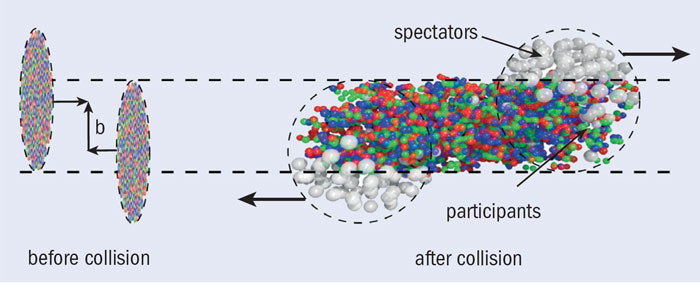
\includegraphics[width=10.0cm]{CCfir5_04_13}
\centering
\caption{Nuclear collison  .}
\label{fig:centrality}
\end{figure}

\noindent
In nuclear collisions the offset between the centers of two nuclei is known as the impact parameter (b) as seen in Figure \ref{fig:centrality}.  Measuring the impact parameter in an experimental setting is non-trivial and model-dependent.  The distribution of nucleons in the nucleus is modeled after a Glauber distribution\cite{Loizides:2016djv}.  The Glauber model predicts that there is a direct correlation between the impact parameter of a nuclear collision and to the inelastic differential cross section ($\sigma_{inel}$)\cite{Miller:2007ri}.


\begin{equation}
c(b) =\frac{ \int_{0}^{b} \frac{d \sigma}{db} db}{ \int_{0}^{\infty} \frac{d \sigma}{db} db} = \frac{1}{\sigma_{inel}} \int_{0}^{b} \frac{d \sigma}{db} db
\label{eq:centrality}
\end{equation}

\fi




\section{The Quark-Gluon Plasma}
Due to asymptotic freedom, the interaction between the partons becomes weaker as $Q^{2}$ increases.  This implies that at some point in the nuclear phase diagram the normal color confinement between the partons 

\subsection{Nuclear Collisions}
By colliding heavy nuclei together in high energy collisions it is possible to obtain the energy densities and temperatures associated with the QGP state.  
\subsection{Jets as a Probe of the QGP}
\subsection{Asymptotic Freedom and the Perfect Fluid}

\subsubsection{Hydrodynamics}
The conservation laws for a relativistic fluid conserve the charge current and energy-momentum tensor of the expanding fluid such that:

\begin{equation}
\partial_{\mu} N_{\textit{i}}^{\mu} = 0
\label{eq:hydrochrg}
\end{equation}

\begin{equation}
\partial_{\mu} T^{\mu \nu} = 0
\label{eq:hydroenrgy}
\end{equation}

\begin{equation}
p_{T}^{jet} = p_{T,rec}^{jet} - \rho A_{jet}
\label{eq:jetsub}
\end{equation}

\noindent
where $p_{T,rec}^{jet}$ is the raw jet $p_{T}$ found by a jet finder, $A_{jet} = \pi R^{2}$ is the jet area, and $\rho$ is the average background energy density per unit area.  $\rho$ is estimated by excluding the two highest momentum particles in a event and using a random cone to find the event-by-event

\section{QGP in Proton-Proton Collisions?}
As previoulsy stated a QGP is believed to be absent in proton-proton collisions, thus any signature of a QGP should likewise be absent.  However, one way of quantifying the presence of the QGP is via the Bjorken energy density.  

\begin{equation}
\varepsilon = \frac{1}{\tau A} \frac{dE_{T}}{d \eta}
\label{eq:bjorkenEt}
\end{equation}

\noindent
where A is the transverse area of the nuclei, $\tau$ is the proper time, and $dE_{T}/d \eta$ is the transverse energy per unit psuedorapidity.  It can be shown that  the 150 MeV critical temperature need for the phase transition to the QGP corresponds to ~ $1 - 3 GeV/fm^{3}$ energy density.  The quantity $dE_{T}/d \eta$ can be related to the mean transverse momentum $<p_{T}>$ and particle multiplictiy\footnote{Multiplicity is defined as the number of particles per event} per unity psuedorapidity as:

\begin{equation}
\frac{dE_{t}}{d \eta}  \approx  <p_{T}> \frac{dN}{d\eta}
\label{eq:Et}
\end{equation}

where $ <p_{T} >$ is the mean transverse momentum and $dN/d\eta$ is the particle multiplicity per unit psuedorapidity.
This suggest that in very high multiplicity proton-proton events signatures of the QGP may be present.  This is one of the most active and newest areas of research in heavy ion physics.  
